\documentclass[11pt]{article}%设置文档类型{article}和字体大小{11pt}，适配本地字体

\usepackage[a4paper]{geometry}%页面布局，纸张大小[a4paper]
\geometry{left=2.0cm,right=2.0cm,top=2.5cm,bottom=2.5cm}%页面边距
\usepackage[UTF8]{ctex}%latex支持中文宏包
\usepackage{amsmath, amsfonts, amssymb, amsthm}%数学公式环境、数学字体、数学字体扩展包、定理环境
\usepackage{bm,mathtools}%数学粗体、amsmath扩展包
\usepackage{graphicx}%插入和管理图片
\usepackage[graphicx]{realboxes}%创建和管理盒子（装有文本和图形）
\usepackage{algorithm,algorithmicx}%支持伪代码宏包
\usepackage[noend]{algpseudocode}%支持伪代码宏包
\usepackage{fancyhdr}%定制页眉和页脚
\setlength{\headheight}{13.6pt}%避免页眉高度警告
\pagestyle{fancy}
\fancyhf{} % 清空默认的页眉和页脚
\fancyhead[L]{\kaishu 中国科学院大学}
\fancyhead[C]{林俊杰2023K8009916012}
\fancyhead[R]{\kaishu}
\fancyfoot[C]{\thepage}
\usepackage{booktabs}%美化表格宏包
\usepackage{caption}%定制图表标题宏包
\usepackage{xcolor}%切换字体颜色
\usepackage{placeins}%控制浮动体位置
\usepackage{cleveref}%智能引用
\crefname{figure}{图}{figures}
\Crefname{figure}{Figure}{Figures}
\crefname{table}{表}{tables}
\Crefname{table}{Table}{Tables}
\usepackage{tikz} % 绘图宏包
\usetikzlibrary{arrows.meta, positioning, calc, shapes, fit, decorations.pathreplacing} % 加载绘图库
\usepackage{tikz-3dplot} %%三维图形绘制需要的宏包
\usetikzlibrary{patterns}%%填充使用的宏包 

%数学环境计数器
\newcounter{counter_exm}\setcounter{counter_exm}{1}
%\newcounter{counter_thm}\setcounter{counter_thm}{1}
%\newcounter{counter_lma}\setcounter{counter_lma}{1}
%\newcounter{counter_dft}\setcounter{counter_dft}{1}
%\newcounter{counter_clm}\setcounter{counter_clm}{1}
%\newcounter{counter_cly}\setcounter{counter_cly}{1}

%图标随章节计数{章节.张数}
\counterwithin{figure}{section}
\counterwithin{table}{section}

\newtheorem{theorem}{{\hskip 1.7em \bf 定理}}
\newtheorem{lemma}[theorem]{\hskip 1.7em 引理}
\newtheorem{proposition}[theorem]{Proposition}
\newtheorem{claim}[theorem]{\hskip 1.7em 命题}
\newtheorem{corollary}[theorem]{\hskip 1.7em 推论}
\newtheorem{definition}[theorem]{\hskip 1.7em 定义}

\renewcommand{\emph}[1]{{\kaishu #1}}
\newcommand{\articlename}{二维坐标系中三角形面积的计算}

\newenvironment{solution}{{\noindent\hskip 2em \bf 解 \quad}}{\par}
\newenvironment{example}{{\noindent\hskip 2em \bf 例 \arabic{counter_exm}\quad}}{\addtocounter{counter_exm}{1}\par}
\newenvironment{concept}[1]{{\bf #1\quad} \begin{kaishu}}{\end{kaishu}\par}
\renewenvironment{proof}{{\noindent\hskip 2em \bf 证明 \quad}}{\hfill$\qed$\par}

\begin{document}
    \begin{center}
        \LARGE \bf \articlename
    \end{center}

    \section{问题描述}

    \begin{figure}[h]
        \centering
        \begin{tikzpicture}[scale=0.8]
            % 坐标轴
            \draw[->] (-0.5,0) -- (7,0) node[right] {$x$};
            \draw[->] (0,-0.5) -- (0,6) node[above] {$y$};

            % 三个点
            \coordinate (A) at (2,1.5);
            \coordinate (B) at (4.5,2.5);
            \coordinate (C) at (3,4.5);

            % 三角形
            \draw[thick] (A) -- (B) -- (C) -- cycle;

            % 顶点
            \fill (A) circle (2pt);
            \fill (B) circle (2pt);
            \fill (C) circle (2pt);

            \node[below] at (A) {$A(x_1,y_1)$};
            \node[right] at (B) {$B(x_2,y_2)$};
            \node[above] at (C) {$C(x_3,y_3)$};

            % 原点
            \node[below left] at (0,0) {$O$};
        \end{tikzpicture}
        \caption{二维坐标系中三角形的顶点}
        \label{fig:1}
    \end{figure}

    如\cref{fig:1}，在二维直角坐标系中，给定三角形的三个顶点
    \[
    A(x_1,y_1)\qquad
    B(x_2,y_2)\qquad
    C(x_3,y_3)
    \]

    如何仅根据三个顶点的坐标，计算三角形 $ABC$ 的面积？
    我们希望找到一种简洁、通用的计算方法，并理解其背后的几何意义。

    \section{解决方法}

    构造三阶行列式
    \[
    \det
    \begin{pmatrix}
    x_1 & x_2 & x_3\\
    y_1 & y_2 & y_3\\
    1   & 1   & 1
    \end{pmatrix}
    \]

    这个行列式的绝对值就等于三角形 $ABC$ 面积的两倍，因此三角形的面积为
    \[
    \boxed{
    S_{ABC}
    =
    \frac{1}{2}
    \left|
    \det
    \begin{pmatrix}
    x_1 & x_2 & x_3\\
    y_1 & y_2 & y_3\\
    1   & 1   & 1
    \end{pmatrix}
    \right|
    }
    \]

    \section{原理讲解}

    \subsection{体积关系}

    \begin{figure}[H]
        \centering
        \tdplotsetmaincoords{70}{110}
        \begin{tikzpicture}[
            tdplot_main_coords,
            scale=0.8,
            ]

            % 绘制六面体
            \coordinate (A) at (0,0,0);
            \coordinate (B) at (4,0,0);
            \coordinate (C) at (4,5,0);
            \coordinate (D) at (0,5,0);
            \coordinate (A') at (0,0,3);
            \coordinate (B') at (4,0,3);
            \coordinate (C') at (4,5,3);
            \coordinate (D') at (0,5,3);

            \draw[thick, dashed] (D) -- (A) -- (B);
            \draw[thick] (A') -- (B') -- (C') -- (D') -- cycle;
            \draw[thick, dashed] (A) -- (A');
            \draw[thick] (B) -- (B');
            \draw[thick] (C) -- (C');
            \draw[thick] (D) -- (D');

            \node[below] at (A) {A};
            \node[below] at (B) {B};
            \node[below] at (C) {C};
            \node[below] at (D) {D};
            \node[above] at (A') {A'};
            \node[above] at (B') {B'};
            \node[above] at (C') {C'};
            \node[above] at (D') {D'};

            % 绘制三棱锥
            \fill[orange!20, opacity=0.8] (C') -- (C) -- (B) -- cycle;
            \fill[orange!20, opacity=0.8] (C') -- (D) -- (B) -- cycle;
            \fill[orange!20, opacity=0.8] (C') -- (C) -- (D) -- cycle;
            \fill[orange!30, opacity=0.8] (C) -- (B) -- (D) -- cycle;

            \draw[thick] (C') -- (C);
            \draw[thick] (C') -- (B);
            \draw[thick] (C') -- (D);
            \draw[thick] (C) -- (B);
            \draw[thick, dashed] (B) -- (D);
            \draw[thick] (D) -- (C);

            % 辅助线
            \draw[thick, dashed] (B') -- (D');
        \end{tikzpicture}
        \caption{三棱锥与六面体}
        \label{fig:2}
    \end{figure}

    考虑三棱柱 $BCD-B'C'D'$，易得它的体积是整个平行六面体体积的 $\frac{1}{2}$。
    
    再考虑三棱柱 $BCD-B'C'D'$ 中的三棱锥 $BCD-C'$，它的体积是三棱柱体积的 $\frac{1}{3}$，
    因此三棱锥 $BCD-C'$ 的体积是整个平行六面体体积的 $\frac{1}{6}$。
    
    也就是说，由平行六面体同一顶点的三条相邻棱所确定的三棱锥的体积是平行六面体的六分之一。

    \[
    \boxed{
    V_{\text{三棱锥}}
    =
    \frac{1}{6}V_{\text{六面体}}
    }
    \]

    \subsection{两种方法计算三棱锥体积}

    \begin{figure}[H]
        \centering
        \tdplotsetmaincoords{70}{110}
        \begin{tikzpicture}[
            tdplot_main_coords,
            scale=1,
            line join=round,
            line cap=round
            ]

            \coordinate (O) at (0,0,0);
            \coordinate (A) at (-1,1,1);
            \coordinate (B) at (-1,-2,1);
            \coordinate (C) at (1,0,1);
            \coordinate (D) at ($(A)+(B)$);
            \coordinate (E) at ($(A)+(C)$);
            \coordinate (F) at ($(B)+(C)$);
            \coordinate (G) at ($(A)+(B)+(C)$);

            % 填充
            \fill[orange!20, opacity=0.8] (O) -- (C) -- (B) -- cycle;
            \fill[orange!20, opacity=0.8] (O) -- (A) -- (B) -- cycle;
            \fill[orange!20, opacity=0.8] (O) -- (C) -- (A) -- cycle;
            \fill[orange!30, opacity=0.8] (C) -- (B) -- (A) -- cycle;

            % 连线
            \draw[thick, dashed] (D) -- (A);
            \draw[thick, dashed] (D) -- (B);
            \draw[thick, dashed] (D) -- (G);
            \draw[thick] (E) -- (A);
            \draw[thick] (E) -- (C);
            \draw[thick] (E) -- (G);
            \draw[thick] (F) -- (B);
            \draw[thick] (F) -- (C);
            \draw[thick] (F) -- (G);
            \draw[thick] (O) -- (A);
            \draw[thick] (O) -- (B);
            \draw[thick] (O) -- (C);
            \draw[thick, dashed] (A) -- (B);
            \draw[thick] (B) -- (C);
            \draw[thick] (C) -- (A);

            % 绘制顶点
            \fill (O) circle (1.8pt);
            \fill (A) circle (1.8pt);
            \fill (B) circle (1.8pt);
            \fill (C) circle (1.8pt);

            % 标注顶点
            \node[below right] at (O) {$O$};
            \node[right] at (A) {$A$};
            \node[left] at (B) {$B$};
            \node[above] at (C) {$C$};

            
            % 绘制坐标轴
            \draw[->] (-0.5,0,0) -- (4.5,0,0) node[below left] {$x$};
            \draw[->] (0,-2.5,0) -- (0,3,0) node[right] {$y$};
            \draw[->] (0,0,-0.3) -- (0,0,4) node[above] {$z$};
        \end{tikzpicture}
        \caption{三角形 $ABC$ 在平面 $z=1$ 上}
        \label{fig:tetrahedron-3d}
    \end{figure}

    如\cref{fig:tetrahedron-3d}，三角形 $ABC$ 的三个顶点均位于平面 $z=1$ 上，因此，从点 $O$ 到平面 $ABC$ 的距离为 $1$。根据三棱锥的体积公式，三棱锥 $OABC$ 的体积为
    \[
    V_{\text{三棱锥}} = \frac{1}{3} \cdot S_{ABC} \cdot h = \frac{1}{3} \cdot S_{ABC} \cdot 1 = \frac{1}{3} S_{ABC}
    \]

    另一方面，平行六面体的体积可以通过行列式表示为
    \[
    V_{\text{六面体}}
    =
    \left|
    \det
    \begin{pmatrix}
    x_1 & x_2 & x_3\\
    y_1 & y_2 & y_3\\
    1 & 1 & 1
    \end{pmatrix}
    \right|
    \]

    而三棱锥 $OABC$ 的体积是平行六面体体积的 $\frac{1}{6}$，因此
    \[
    V_{\text{三棱锥}}
    =
    \frac{1}{6}
    \left|
    \det
    \begin{pmatrix}
    x_1 & x_2 & x_3\\
    y_1 & y_2 & y_3\\
    1 & 1 & 1
    \end{pmatrix}
    \right|
    \]

    由于以上两种方法计算的是同一个三棱锥的体积，因此
    \[
    \frac{1}{3}S_{ABC}
    =
    \frac{1}{6}
    \left|
    \det
    \begin{pmatrix}
    x_1 & x_2 & x_3\\
    y_1 & y_2 & y_3\\
    1 & 1 & 1
    \end{pmatrix}
    \right|
    \]

    于是得到
    \[
    \boxed{
    S_{ABC}
    =
    \frac{1}{2}
    \left|
    \det
    \begin{pmatrix}
    x_1 & x_2 & x_3\\
    y_1 & y_2 & y_3\\
    1 & 1 & 1
    \end{pmatrix}
    \right|
    }
    \]
    最终我们得到了二维坐标系中三角形面积的计算公式。

    \section{三阶行列式的计算}

    \[
    \det
    % 一个3*3矩阵
    \begin{pmatrix}
    a_{11} & a_{12} & a_{13}\\
    a_{21} & a_{22} & a_{23}\\
    a_{31} & a_{32} & a_{33}
    \end{pmatrix}
    % 计算结果太长，给我分行
    =
    a_{11}a_{22}a_{33}+a_{12}a_{23}a_{31}+a_{13}a_{21}a_{32}-a_{31}a_{22}a_{13}-a_{32}a_{23}a_{11}-a_{33}a_{21}a_{12}
    \]

    上面的公式不便记忆，因此我们可以使用图形化的方法来记忆三阶行列式的计算方法。

    \begin{figure}[H]
        \centering
        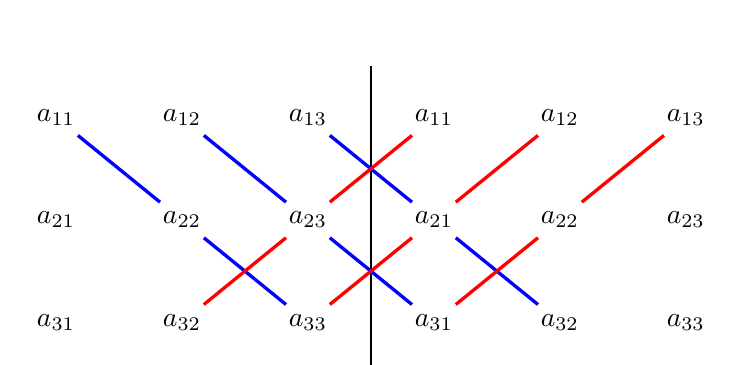
\begin{tikzpicture}[
            x=1.6cm,
            y=1.3cm,
            >=stealth
            ]

            % 原矩阵
            \node (a11) at (0,3) {$a_{11}$};
            \node (a12) at (1,3) {$a_{12}$};
            \node (a13) at (2,3) {$a_{13}$};

            \node (a21) at (0,2) {$a_{21}$};
            \node (a22) at (1,2) {$a_{22}$};
            \node (a23) at (2,2) {$a_{23}$};

            \node (a31) at (0,1) {$a_{31}$};
            \node (a32) at (1,1) {$a_{32}$};
            \node (a33) at (2,1) {$a_{33}$};

            % 复制矩阵
            \node (a11') at (3,3) {$a_{11}$};
            \node (a12') at (4,3) {$a_{12}$};
            \node (a13') at (5,3) {$a_{13}$};

            \node (a21') at (3,2) {$a_{21}$};
            \node (a22') at (4,2) {$a_{22}$};
            \node (a23') at (5,2) {$a_{23}$};

            \node (a31') at (3,1) {$a_{31}$};
            \node (a32') at (4,1) {$a_{32}$};
            \node (a33') at (5,1) {$a_{33}$};

            % 分割线
            \draw[thick] (2.5,0.5) -- (2.5,3.5);

            % 对角线
            \draw[blue, very thick] (a11) -- (a22) -- (a33);
            \draw[blue, very thick] (a12) -- (a23) -- (a31');
            \draw[blue, very thick] (a13) -- (a21') -- (a32');
            \draw[red, very thick] (a31') -- (a22') -- (a13');
            \draw[red, very thick] (a32) -- (a23) -- (a11');
            \draw[red, very thick] (a33) -- (a21') -- (a12');
        \end{tikzpicture}
        \caption{三阶行列式的计算方法}
        \label{fig:det3x3}
    \end{figure}

    如\cref{fig:det3x3}，我们将矩阵复制到右侧，
    然后按照图中蓝色的三条对角线方向相乘并求和，得到行列式的正项；
    按照图中红色的三条副对角线方向相乘并求和，得到行列式的负项。
    最终将正项减去负项，就得到了三阶行列式的计算结果。
\end{document}